\documentclass{beamer}
% beamer settings
\usetheme{Custom}
\usefonttheme{professionalfonts} % make beamer work best with unicode-math
% \usefonttheme[stillsansserifsmall,stillsansseriflarge]{serif}
\setbeamercovered{transparent}

% Delete this, if you do not want the table of contents to pop up at
% the beginning of each subsection:
\AtBeginSubsection[]
{
  \begin{frame}<beamer>{Outline}
    \tableofcontents[currentsection,subsectionstyle=show/shaded/hide]
  \end{frame}
}

% microtype for improved spacing and readability
\usepackage{microtype}

% language stuff
% \usepackage{polyglossia}
% \setdefaultlanguage[variant=american]{english}
\usepackage[english=american]{csquotes} % english=american needed because polyglossia support is not good yet
\MakeOuterQuote{"}
\MakeAutoQuote{<}{>}

% modern font stuff
\usepackage{fontspec} % enable access to system fonts
% Mapping=tex-text not supported yet in LuaTeX
% \defaultfontfeatures{Mapping=tex-text} % map TeX conventions for quotation marks, dashes to proper characters
\defaultfontfeatures{Ligatures=TeX} % map TeX conventions for quotation marks, dashes to proper characters
%\setmainfont{STIXGeneral}
%\setmainfont{Times New Roman}
%\setmainfont{Linux Libertine O} % open source Times New Roman look-alike
\setmainfont{TeX Gyre Pagella} % expanded URW Palladio, like Palatino
%\setsansfont{TeX Gyre Adventor} % expanded URW Gothic, like AvantGarde
\setsansfont[Scale=MatchLowercase]{Linux Biolinum} % similar to Optima/URW Classico which pairs well with Palatino
% \setsansfont[Scale=MatchLowercase]{Linux Biolinum O} % similar to Optima/URW Classico which pairs well with Palatino
%\setmonofont{}
%\usepackage{unicode-math}
%\setmathfont{Latin Modern Math}
%\setmathfont{xits-math.otf} % use with Times
%\setmathfont{Asana-Math.otf} % use with Palatino/URW Palladio/TeXGyrePagella

% graphics
\usepackage{graphicx}
\DeclareGraphicsExtensions{.pdf,.png,.jpg}
\graphicspath{{../figures/}}
\usepackage{tikz,ifthen}
\tikzstyle{image}=[inner sep=0pt]
% includecoveredgraphics and covergraphics commands to enable image transparency
\makeatletter
\let\includecovered@origgraphics=\includegraphics
\newcommand{\includecoveredgraphics}[2][]{%
    \ifthenelse{\the\beamer@coveringdepth=1}{%
        \tikz{
          \begin{scope}[opacity=0.6,transparency group]
            \node[inner sep=0pt,outer sep=0pt]
                {\includecovered@origgraphics[#1]{#2}};
          \end{scope}
        }%
    }{%
        \tikz
            \node[inner sep=0pt,outer sep=0pt]
                {\includecovered@origgraphics[#1]{#2}};%
    }%
}
\renewcommand<>{\includecoveredgraphics}[2][]{\onslide#3{\beameroriginal{\includecoveredgraphics}[#1]{#2}}}
\def\covergraphics{\def\includegraphics{\includecoveredgraphics}}
\makeatother

% other packages
\usepackage{tikz}
\usepackage[absolute,overlay]{textpos}
\TPGrid{1}{1}
\usepackage{mathtools} % for math stuff not provided by AMSmath
\usepackage{multimedia} % movies
\usepackage{appendixnumberbeamer} % do not include appendix slides in total frame number

% define commands
\DeclareMathOperator*{\argmin}{arg\,min}
%\DeclareMathSymbol{\Sha}{\mathalpha}{cyrletters}{"58}
\DeclarePairedDelimiter{\abs}{\lvert}{\rvert}
\DeclarePairedDelimiter{\nrm}{\lVert}{\rVert}
%\DeclarePairedDelimiterX{\innerprod}[2]{\langle}{\rangle}{#1, #2}
\usepackage{mathcommands-private}

%%%%%%%%%%%%%%%%%%%%%%%%%%%%%%%%%%%%%%%%%%%%%%%%%%%%%%%%%%%%%%%%%%%%%%%%%%%%%%%

\title[Sparsity for Ionospheric Radar]{Theory and Applications of Sparsity\\for Radar Sensing of Ionospheric Plasma}
\author{Ryan Volz}
\institute[Stanford University]
{
	Department of Aeronautics and Astronautics\\
	Stanford University
}
\date{}

\begin{document}

{
% % center page when using a plain frame
% \makeatletter
% \setlength{\hoffset}{.5\beamer@sidebarwidth}
% \makeatother
\begin{frame}[plain]
 \begin{columns}
  \column{0.25\textwidth}
  \centering
\includegraphics[width=\textwidth]{stanford_aero_astro}
  \column{0.5\textwidth}
  \centering
\includegraphics[width=0.75\textwidth]{sess_logo_custom}
  \column{0.25\textwidth}
  \centering
\includegraphics[width=0.75\textwidth]{SU_Seal_Card_pos}
 \end{columns}
 \titlepage
\end{frame}
}

\section*{Introduction and Motivation}
\subsection*{The Ionosphere}

\begin{frame}{What is the ionosphere?}
 \includegraphics<1>[width=\textwidth]{atmospheric_regions}
 \includegraphics<2>[width=\textwidth]{atmospheric_regions_with_ionosphere}
 \includegraphics<3>[width=\textwidth]{atmospheric_regions_with_radiation}
 \begin{center}
  \tiny
  Image from NSF (2011), CEDAR: The New Dimension
 \end{center}
  
 \begin{textblock}{0.47}(0.25,0.48)
  \visible<2>{
   \begin{definition}
    The \alert{ionosphere} is a region of \alert{partially ionized gas (plasma)} that envelops the Earth from an altitude of about 60 km and higher.
   \end{definition}
  }
 \end{textblock}
 \begin{textblock}{0.47}(0.25,0.48)
  \visible<3->{
   \begin{block}{Mechanism}
    Ionization is principally caused by solar radiation.
   \end{block}
  }
 \end{textblock}
\end{frame}

\begin{frame}<1-2>[label=ionosphere_importance]{Importance of the ionosphere}
 \only<1,3>{
  \begin{block}<1>{Communications}
   \begin{itemize}
    \item Radio waves of lower frequency (less than $\approx 10$\ MHz) reflect off ionosphere.
    \item Microwave frequencies (e.g. GPS) can pass through, but experience frequency-dependent refraction and delay.
    \item Plasma irregularities additionally perturb signals.
   \end{itemize}
  \end{block}
  \begin{block}<3>{Coupling between Earth and space}
   \begin{itemize}
    \item Space environment (e.g. meteors) can be measured.
    \item Global processes (e.g. weather) are affected by ionosphere.
   \end{itemize}
  \end{block}
 }
 \only<2>{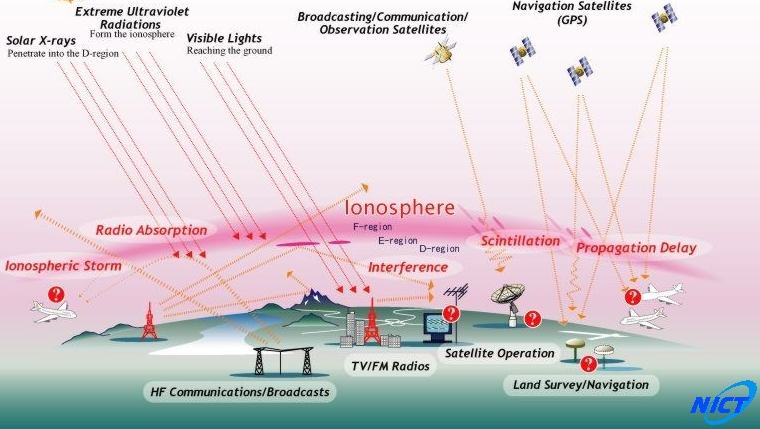
\includegraphics[width=\textwidth]{ionosphere_communications}}
 \only<4>{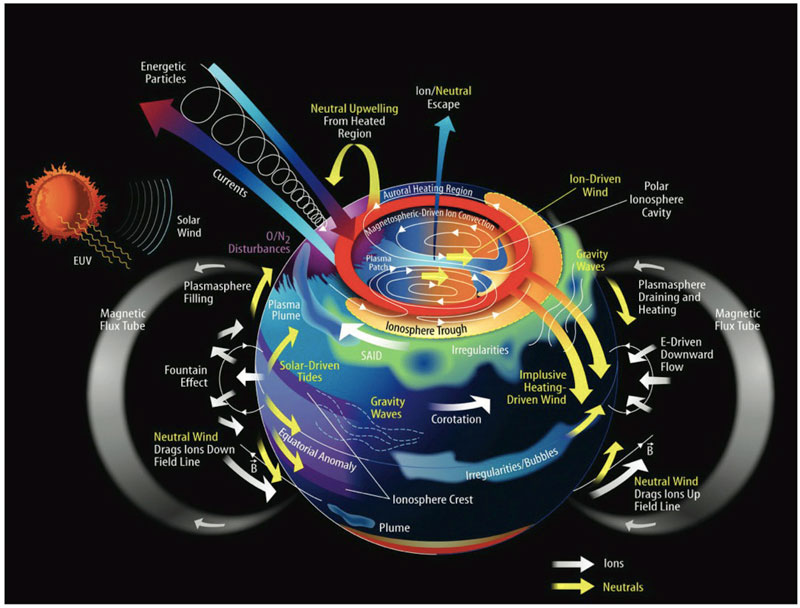
\includegraphics[height=0.9\textheight]{ionosphereprocesses}}
\end{frame}

\againframe<3-4>{ionosphere_importance}

\subsection*{Ionospheric Radar}

\begin{frame}{Measuring the ionosphere}
 \begin{definition}
  \alert{Incoherent Scatter Radars} (ISRs, locations shown {\color{red}below}) are radars sensitive enough to measure scattering from electrons in the background ionosphere.
 \end{definition}
 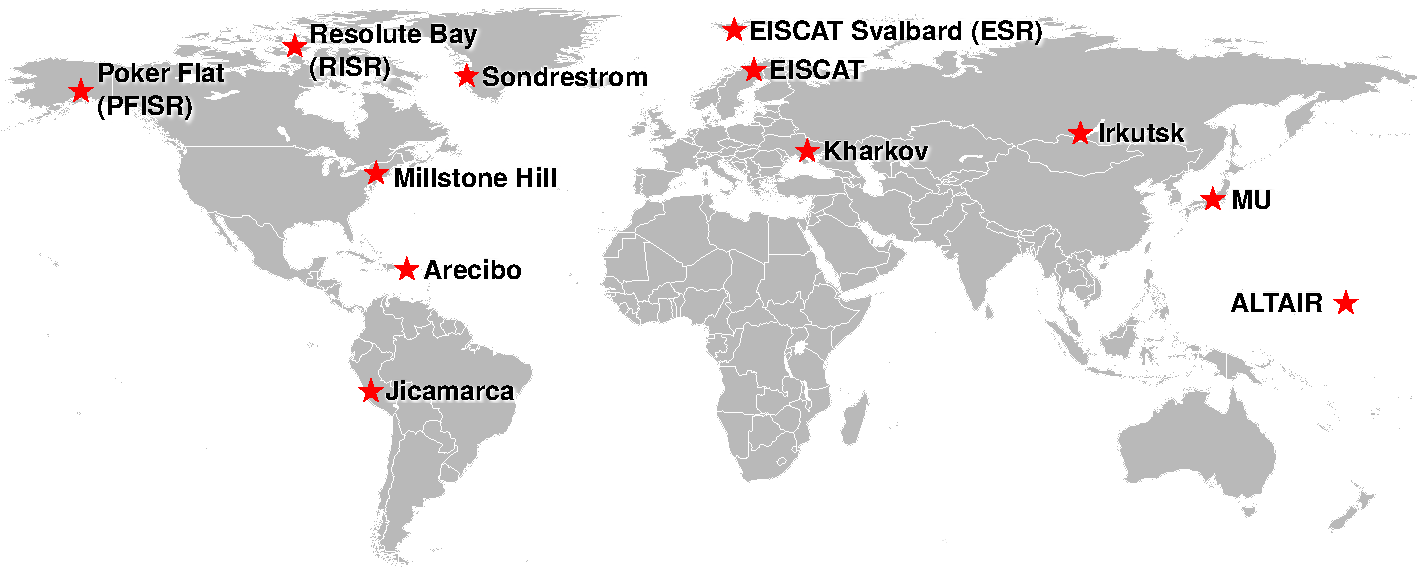
\includegraphics[width=\textwidth]{isr_map}
 \begin{textblock}{0.5}(0.425,0.475)
  \only<2>{
  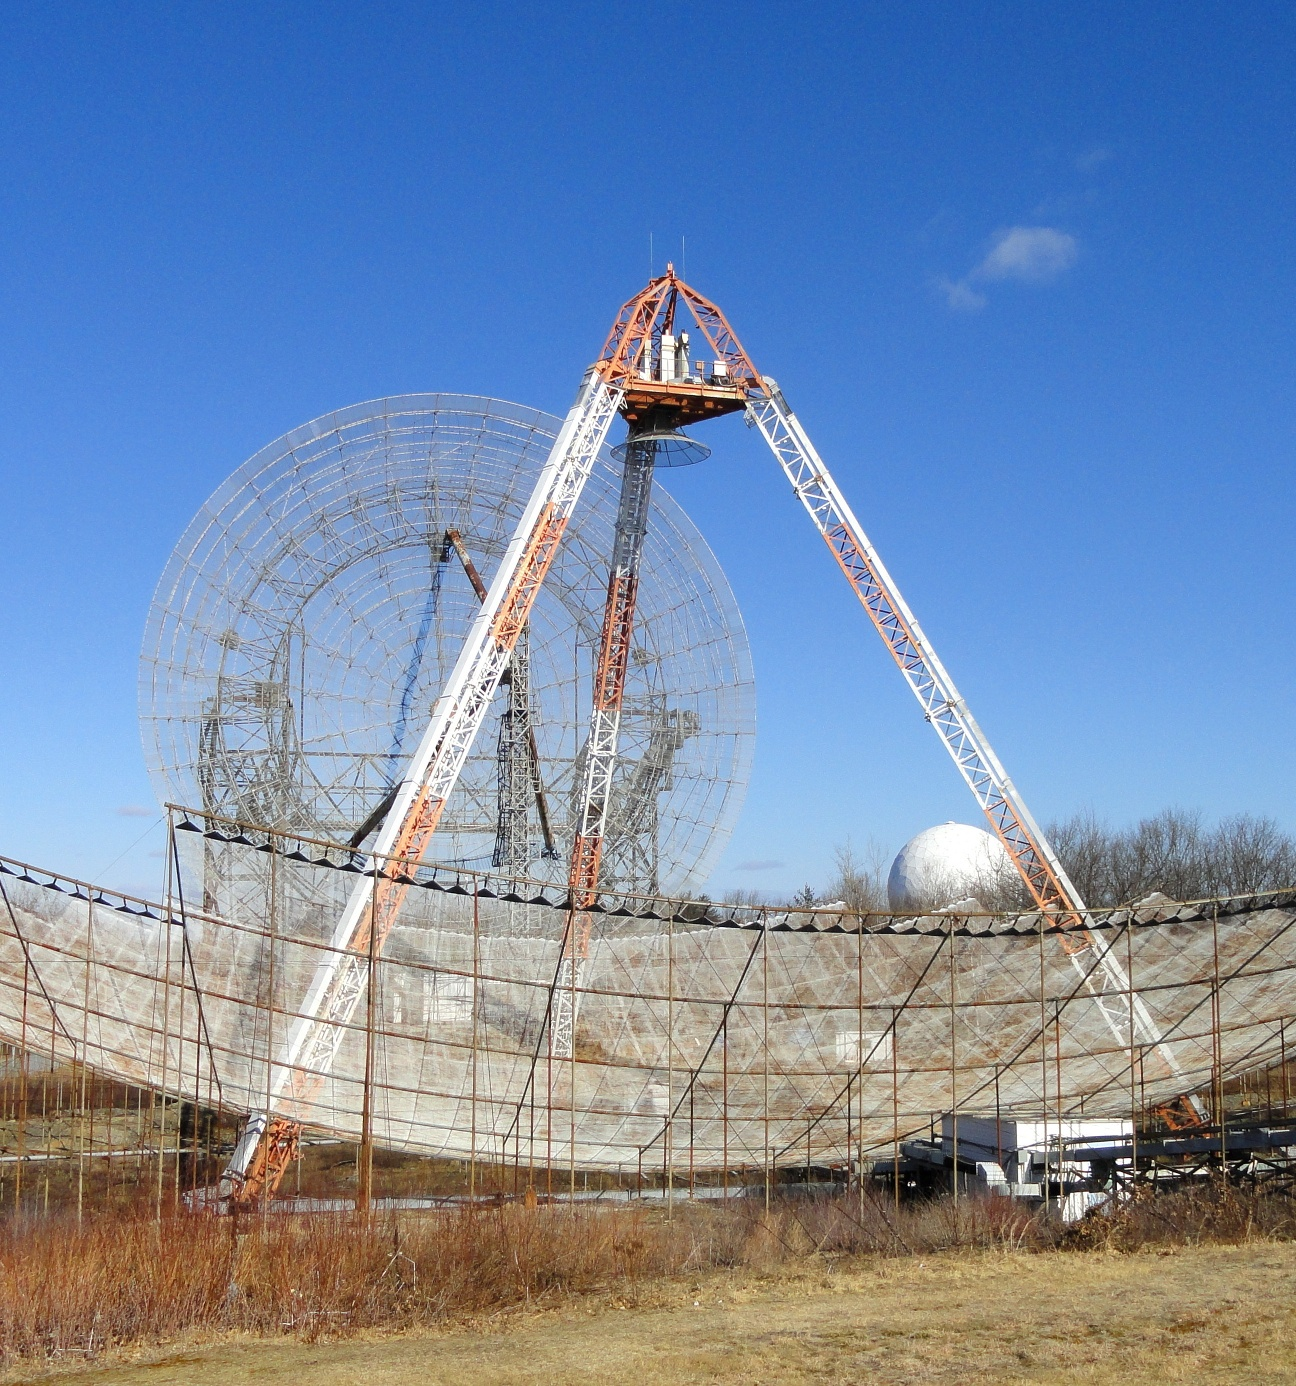
\includegraphics[height=4.75cm]{millstone_hill_radar}\\
  \vspace{-4.75cm}\ \textbf{Millstone Hill}
  }
 \end{textblock}
 \begin{textblock}{0.5}(0.425,0.6)
  \only<3>{
  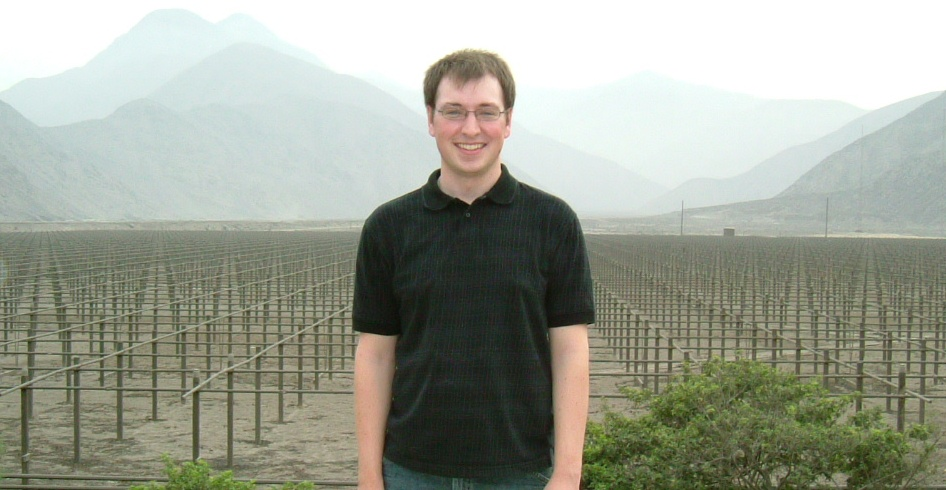
\includegraphics[height=3.6cm]{jicamarca_and_me}\\
  \vspace{-3.6cm}\ \textbf{Jicamarca}
  }
 \end{textblock}
\end{frame}

\begin{frame}{Zoo of ionospheric plasma}
 There are many different plasma phenomena, each presenting its own challenges for observation.
 \begin{columns}
  \column{0.365\textwidth}
  \begin{itemize}
   \item Background ionosphere
   \item {\color{green!80!black}Electrojet}
   \item {\color{yellow!90!black}Meteor}
   \item Spread F
   \item Sporadic E
   \item Equatorial plumes/bubbles
   \item "150-km" echoes
   \item Polar Mesospheric Summer Echoes
  \end{itemize}
  \column{0.635\textwidth}
  \\
  \begin{beamercolorbox}[center]{example text}
   Example data from Jicamarca
  \end{beamercolorbox}
  \begin{tikzpicture}[thick]
   \node[above right] at (0,0) {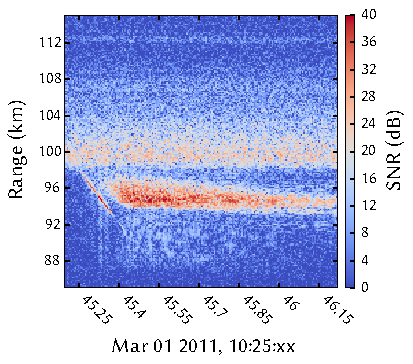
\includegraphics{ejet_head_flare_mf_rti_3}};
   \draw[green!80!black] (1.225,3.4) rectangle (5.97,4.25);
   \draw[yellow!90!black] (1.5,2.6) rectangle (5.97,3.375);
  \end{tikzpicture}
 \end{columns}
\end{frame}

\begin{frame}{Meteors}
 \begin{definition}
  A \alert{meteor} is the plasma (ionized gas) that is created when a meteoroid (small space object) enters the atmosphere.
 \end{definition}
 \begin{block}{Types of scattering}
 \vspace{-0.5em}
  \begin{itemize}
   \item {\color{green!80!black}Head}: dense ball of plasma surrounding the meteoroid
   \item {\color{yellow!90!black}Trail}: plasma left in wake of meteoroid
  \end{itemize}
  \centering
  \vspace*{-0.75em}
  \begin{tikzpicture}[thick]
   \node[above right] at (0,0) {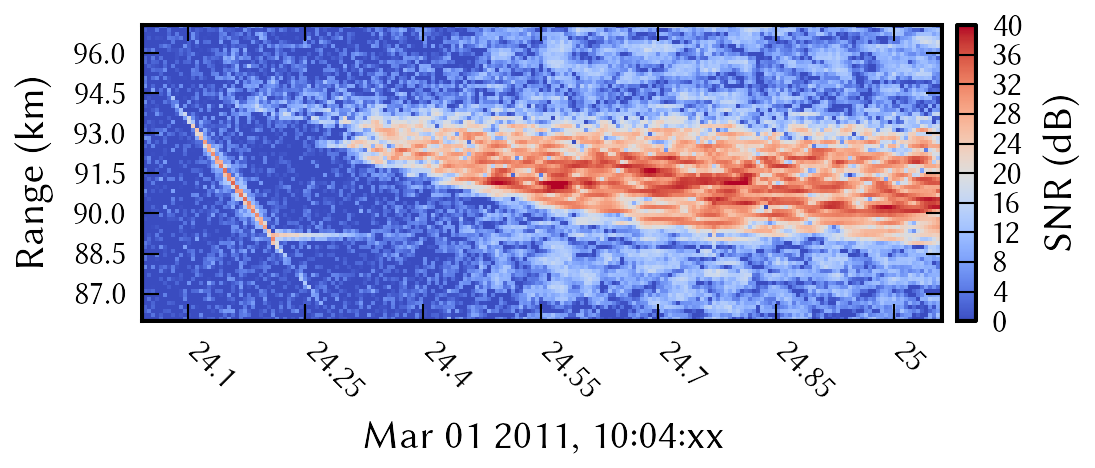
\includegraphics{head_and_flare_mf_rti_3}};
   \draw[yellow!90!black] (2.8,2) rectangle (8.2,3.25);
   \draw[green!80!black,shift={(2.2,2.45)},rotate=-55] (-1.2,-0.15) rectangle (1.2,0.15);
  \end{tikzpicture}
  \vspace*{-0.75em}
 \end{block}
\end{frame}

\begin{frame}{Competing demands on radar measurements}
 Some requirements favor a shorter radar pulse, while others favor a longer radar pulse.
 \begin{columns}
  \column{0.5\textwidth}
  \begin{block}{Short pulse}
   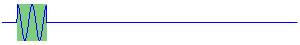
\includegraphics[width=\textwidth]{shortpulse}
   \begin{itemize}
    \item Low range ambiguity
    \item Simple to interpret
   \end{itemize}
  \end{block}
  \column{0.5\textwidth}
  \begin{block}{Long pulse}
   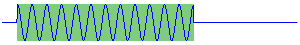
\includegraphics[width=\textwidth]{longpulse}
   \begin{itemize}
    \item Fine frequency resolution
    \item High total power
   \end{itemize}
  \end{block}
 \end{columns}
\end{frame}

\begin{frame}{Coded pulses}
 \begin{itemize}
  \item Encoding allows long pulses to have the low range ambiguity of short pulses.
  \item One method: divide pulse into \alert{bauds} of constant phase.
 \end{itemize}
 \begin{exampleblock}{Barker-13 code}
  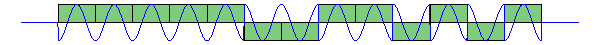
\includegraphics[width=\textwidth]{barker13pulse}
 \end{exampleblock}
 \begin{exampleblock}{Minimum peak sidelobe code}
  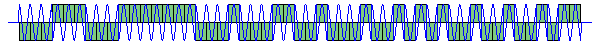
\includegraphics[width=\textwidth]{mslpulse}
 \end{exampleblock}
 \begin{exampleblock}{Linear frequency modulation (LFM chirp)}
  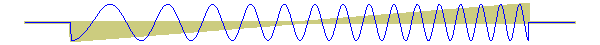
\includegraphics[width=\textwidth]{lfmpulse}
 \end{exampleblock}
\end{frame}

\subsection*{The Problem}

\begin{frame}{Delay-frequency sidelobes}
 Unfortunately, decoding poses its own ambiguity problem that adds complexity to analysis: \alert{delay-frequency sidelobes}.
 \begin{tikzpicture}
  \tikzstyle{every node}=[minimum width=\widthof{Near-ideal}+2ex]
  \node<1>[left,align=center] at (0,0.5) {Uncoded};
  \node<1>[right,image] at (0,0) {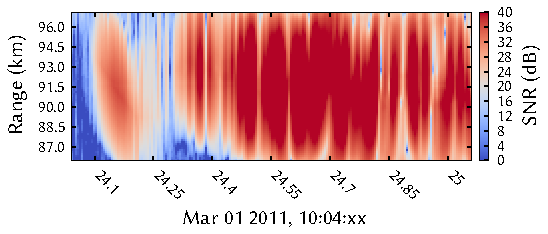
\includegraphics{head_and_flare_mf_rti_2}};
  \node<2>[left,align=center] at (0,0.5) {Near-ideal\\decoding};
  \node<2>[right,image] at (0,0) {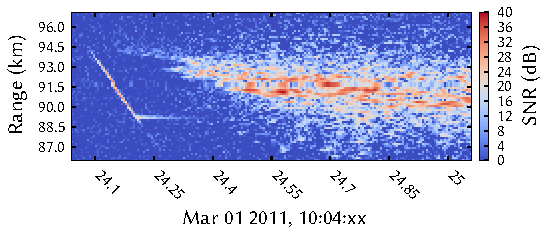
\includegraphics{head_and_flare_recovered_rti_noise_1}};
  \fill[white] (0,-1.125) rectangle (9,-0.875);
  \node[left,align=center] at (0,-2.3) {Minimum\\sidelobe\\code};
  \node[right,image] at (0,-2.8) {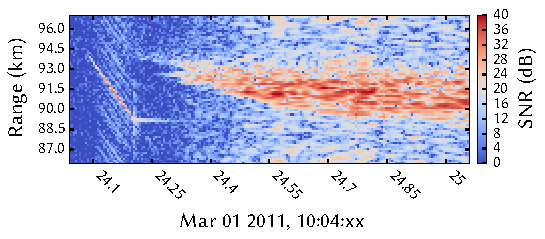
\includegraphics{head_and_flare_mf_rti_1}};
 \end{tikzpicture}
\end{frame}

\begin{frame}{Sidelobe limitations examples: meteors}
 \begin{exampleblock}{Fragmentation}
  \begin{columns}[onlytextwidth]
   \column{0.6\textwidth}
   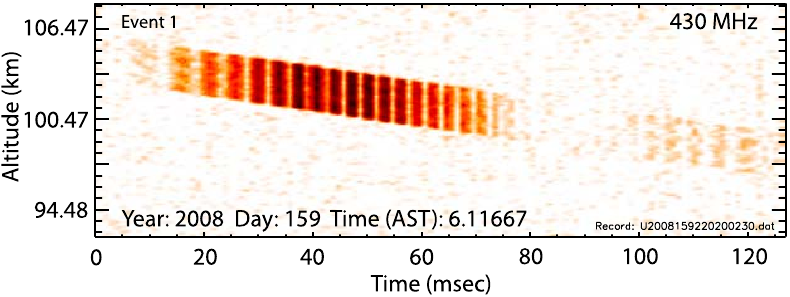
\includegraphics[width=\textwidth]{mathews_fragmentation}
   \column{0.39\textwidth}
   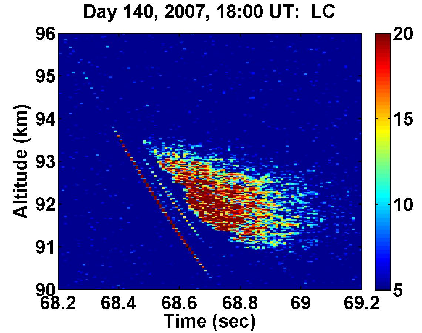
\includegraphics[width=\textwidth]{altair_multiple_scatterers}
  \end{columns}
 \end{exampleblock}
 \begin{exampleblock}{Flares and terminal events}
  \centering
  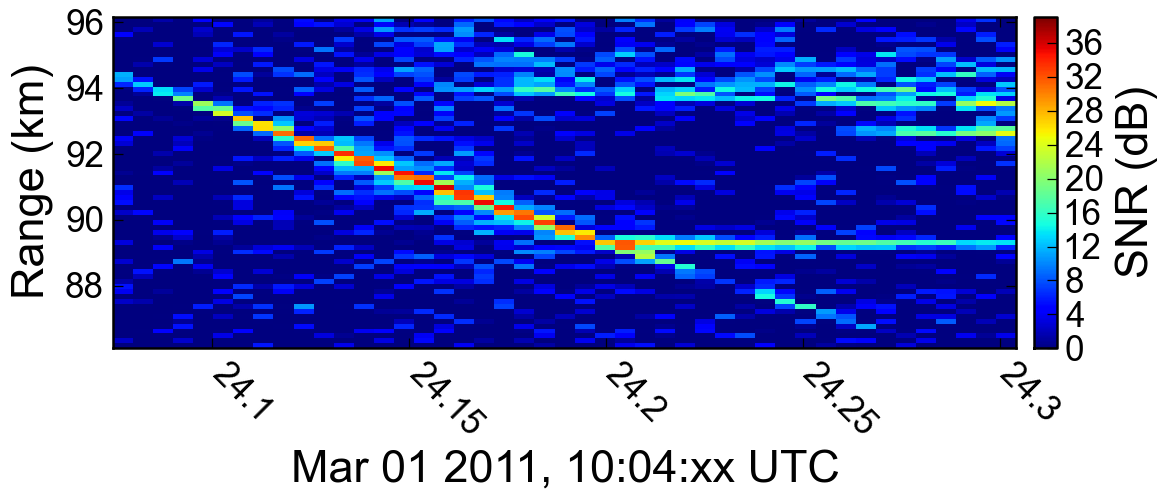
\includegraphics[width=0.6\textwidth]{jicamarca_intro_flare}
 \end{exampleblock}
\end{frame}

\begin{frame}{Sidelobe mitigation}
 \begin{block}{Delay-frequency sidelobe mitigation in use}
  \begin{itemize}
   \item Careful code selection and \alert{ignoring remaining sidelobes}
   \item Sub-optimal inverse filters
   \item Multiple-pulse alternating codes
  \end{itemize}
 \end{block}
 These strategies severely constrain the \alert{flexibility} and \alert{accuracy} of ionospheric radar measurements!
 \begin{block}{Perfect decoding is hard}
  \begin{itemize}
   \item Inversion is complex, filtering is simple
   \item Infinite number of ways to decode and get a target scene that reproduces the measurements
  \end{itemize}
 \end{block}
\end{frame}

\begin{frame}{Sparsity to the rescue}
 How do we visually ignore sidelobes in simple cases? \alert{Sparsity}
 \begin{center}
  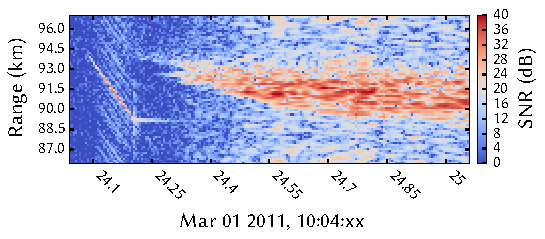
\includegraphics{head_and_flare_mf_rti_1}
 \end{center}
 Radar targets are typically sparse in range and frequency!
 \begin{center}
  \begin{minipage}{0.7\textwidth}
   \begin{alertblock}{}<2->
    \centering
    Can use sparsity to systematically remove sidelobes and achieve perfect decoding
   \end{alertblock}
  \end{minipage}
 \end{center}
\end{frame}

\subsection*{}

\begin{frame}<1-4>[label=contributions]{Contributions}
 \begin{enumerate}
  \item<1,5-> Radar model
  \item<2,6-> Analysis of sparsity and model representation
  \item<3,7-> Efficient implementation of inversion
  \item<4,8-> Detection and classification algorithms
 \end{enumerate}
\end{frame}

\begin{frame}{Outline}
 \tableofcontents[hideallsubsections]
\end{frame}

\section{Development of Radar Model}
\subsection{Matched Filtering}

\begin{frame}{The matched filter}
 \begin{definition}
  The \alert{matched filter} correlates every segment of the received signal with the transmitted pulse.
 \end{definition}
 \begin{example}[Barker-13 code]
 \end{example}
 \centering
 \movie[autostart,loop,poster,width=4in,height=1.501730in]{}{autocorrelation_animation_b13.mp4}
\end{frame}

\begin{frame}{Classical detection with the matched filter}
 \begin{block}{Ideal point target}
  \begin{itemize}
   \item Point target perfectly reflects the transmitted signal
   \item Receive attenuated copy of signal after some delay
   \item Delay is a function of the target's range
  \end{itemize}
 \end{block}
 \begin{block}{Matched filter properties}
  \begin{itemize}
   \item Peak of output gives \alert{maximum likelihood estimate} of target's range and amount of attenuation
   \item Maximum signal-to-noise ratio (SNR) at peak of all filters
  \end{itemize}
 \end{block}
\end{frame}

\begin{frame}{Frequency filter banks}
 \begin{block}{Doppler frequency shift}
  If the target is moving {\color{blue}toward} or {\color{red}away from} the radar, the reflected signal is frequency shifted {\color{blue}up} or {\color{red}{down}}.
 \end{block}
 \begin{itemize}
  \item Matched filter needs to be similarly frequency shifted
  \item True frequency shift is not known ahead of time
  \item Process signal with a bank of differently-shifted filters
 \end{itemize}
 \begin{columns}
  \column{0.5\textwidth}
  \centering
  Result of filter bank\\for ideal reflection,\\using Barker-13 code
  \column{0.5\textwidth}
  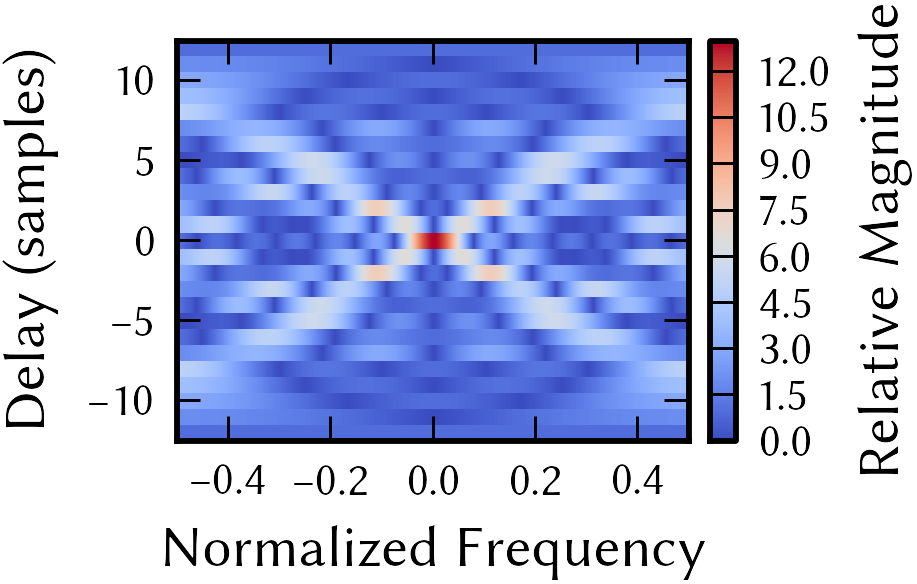
\includegraphics{ambiguity_barker13}
 \end{columns}
\end{frame}

\begin{frame}{Ambiguity functions}
 \begin{definition}
  A delay-frequency \alert{ambiguity function} is produced when a signal is matched against itself using a filter bank.
 \end{definition}
 \begin{columns}
  \column{0.5\textwidth}
  \centering
  Uncoded pulse\\
  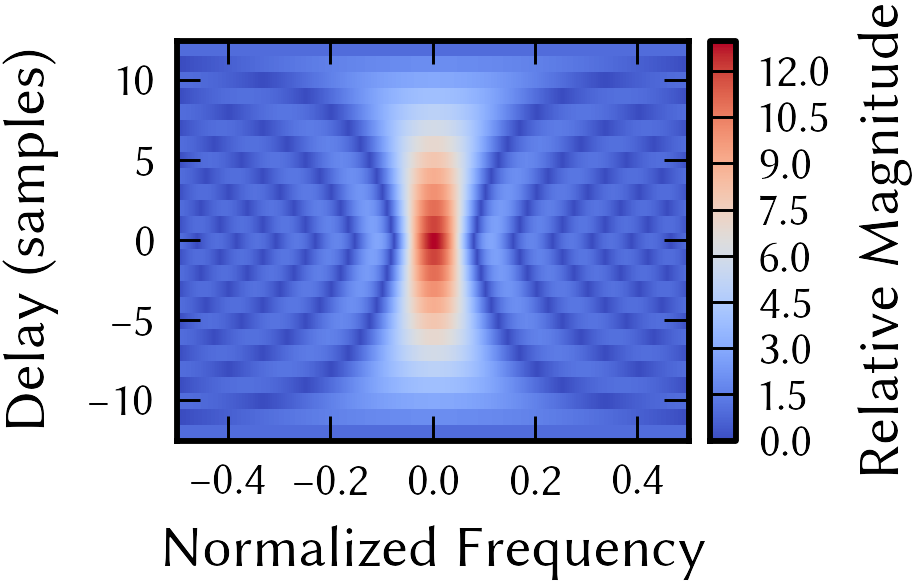
\includegraphics{ambiguity_uncoded}
  \column{0.5\textwidth}
  \centering
  Barker-13\\
  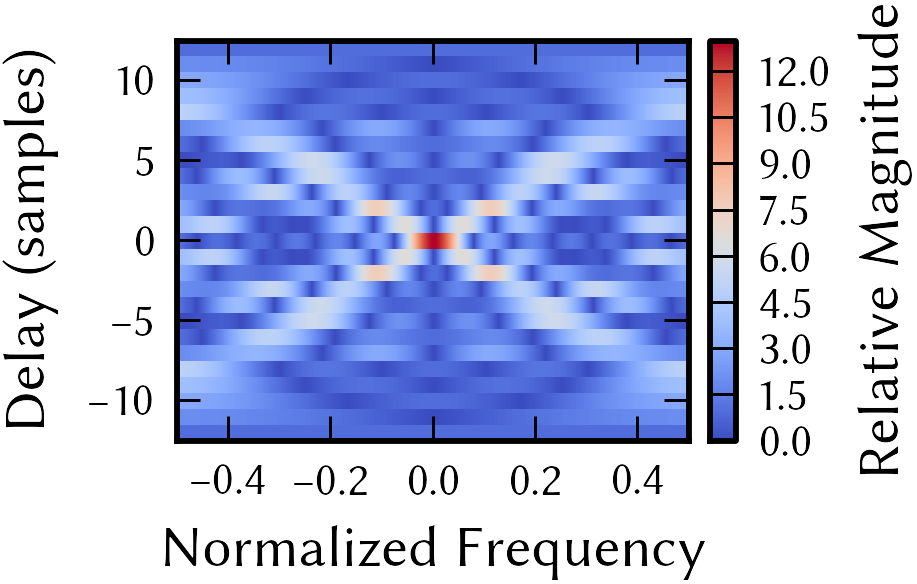
\includegraphics{ambiguity_barker13}
 \end{columns}
 \begin{alertblock}{}
  The ambiguity function describes the delay-frequency sidelobes of a code.
 \end{alertblock}
\end{frame}

\begin{frame}{More example ambiguity functions}
 \begin{columns}
  \column{0.5\textwidth}
  \centering
  Minimum sidelobe\\
  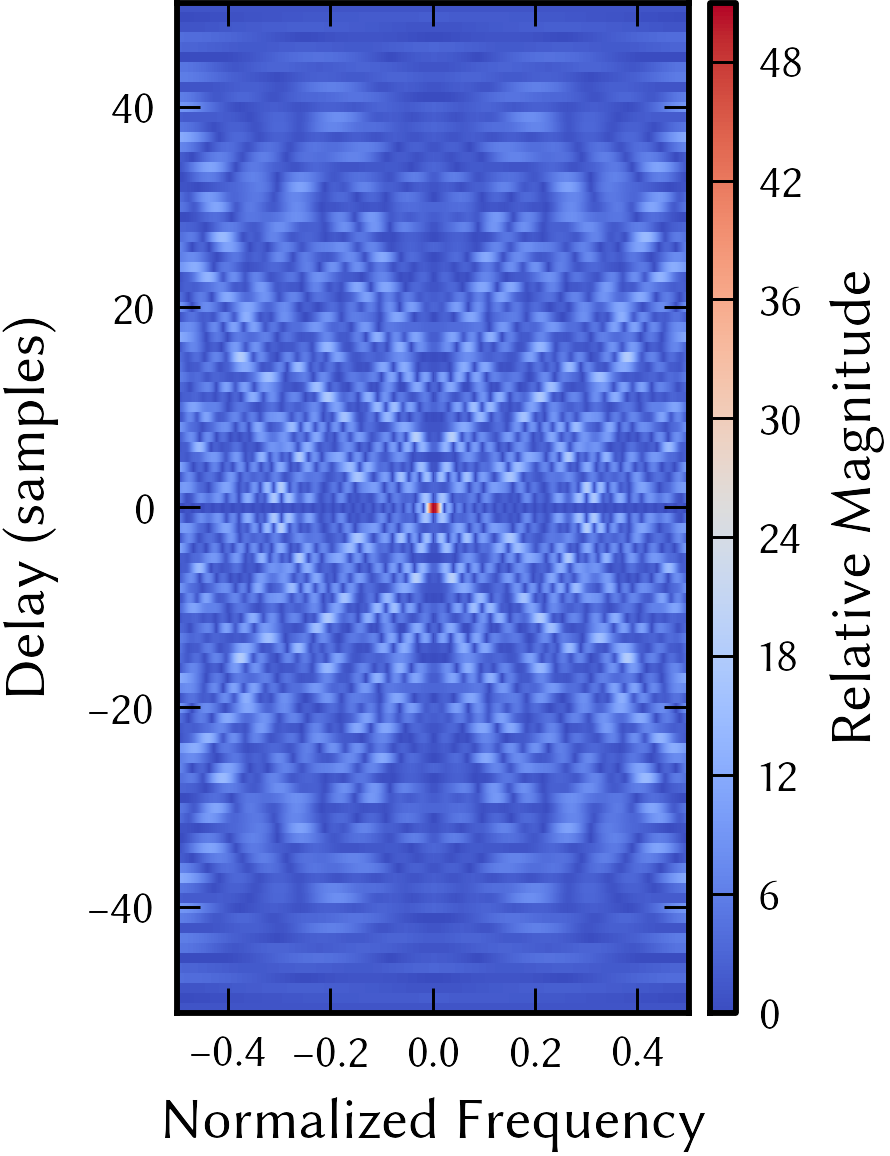
\includegraphics{ambiguity_msl}
  \column{0.5\textwidth}
  \centering
  LFM Chirp\\
  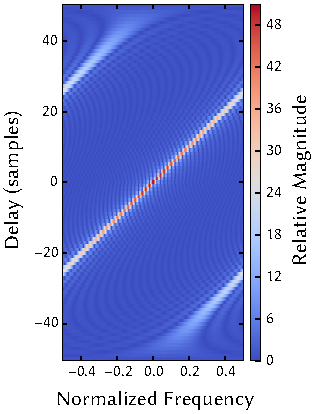
\includegraphics{ambiguity_lfm}
 \end{columns}
\end{frame}

\begin{frame}{Inverse filter ambiguity function}
 \begin{definition}
  The \alert{inverse filter} is designed to produce no delay sidelobes if filtering is done at the target's frequency (for loss of SNR).
 \end{definition}
 \begin{columns}
  \column{0.5\textwidth}
  \centering
  Barker-13 Matched\\
  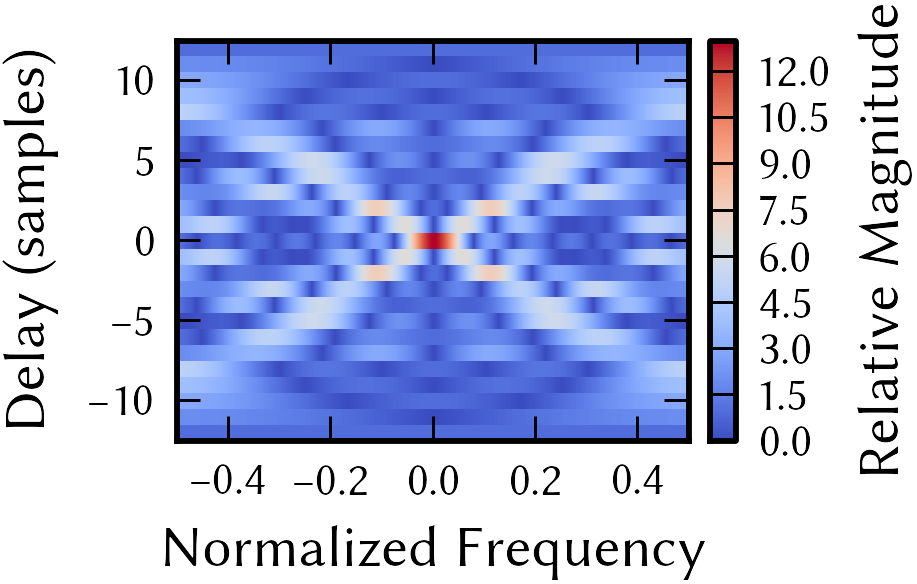
\includegraphics{ambiguity_barker13}
  \column{0.5\textwidth}
  \centering
  Barker-13 Inverse\\
  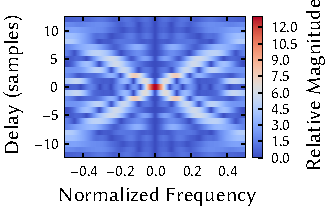
\includegraphics{inverse_ambiguity_barker13}
 \end{columns}
 \begin{alertblock}{}
  No advantage if Doppler shift is unknown or multiple frequencies must be decoded!
 \end{alertblock}
\end{frame}


\subsection{Defining the Model}

\begin{frame}{Matched filtering as imaging}
 \begin{block}{Imaging analogy}
  Measured "image" is blurred by the ambiguity function:
  \begin{equation*}
   {\color{purple}x[n,p]} = {\color{blue}\chi[n,p]} * {\color{red}h[n,p]}
  \end{equation*}
  \vspace{-2ex}
  \begin{columns}[onlytextwidth]
   \column{0.33\textwidth}
   \centering
   {\color{purple}Matched filter result\\(measured image)}
   \column{0.33\textwidth}
   \centering
   {\color{blue}Ambiguity\\function}
   \column{0.33\textwidth}
   \centering
   {\color{red}Target reflectivity\\(source image)}
  \end{columns}
 \end{block}
 (Insert blurring figure)
\end{frame}

\begin{frame}{Towards ambiguity inversion}
 \begin{block}{Ambiguity equation}
  Represent matched filter ambiguity as linear system $X$:
  \begin{equation*}
   x[n,p] = X\left(h[n,p]\right) \quad\longrightarrow \text{Equation is non-invertible.}
  \end{equation*}
 \end{block}
 \begin{block}{Make matched filtering explicit}
  Let $A^*$ represent frequency-shifted matched filtering. Then
  \begin{equation*}
   X(h) = A^*\left(A(h)\right)
  \end{equation*}
  the ambiguity operation is matched filtering composed with its adjoint. Rewrite the ambiguity equation:
  \begin{equation*}
   A^*\left(y[m]\right) = A^*\left(A\left(h[n,p]\right)\right)
  \end{equation*}
 \end{block}
\end{frame}

\begin{frame}{Radar model from matched filter}
 \begin{columns}
  \column{0.5\textwidth}
  \begin{block}{Ambiguity equation}
   \vspace{-2ex}
   \begin{equation*}
    A^*\left(y[m]\right) = A^*\left(A\left(h[n,p]\right)\right)
   \end{equation*}
  \end{block}
  \begin{block}{Radar model}
   Simplify by removing excess matched filtering operation:
   \begin{equation*}
    {\color{purple}y[m]} = {\color{blue}A}\left({\color{red}h[n,p]}\right)
   \end{equation*}
   \vspace{-2ex}
   \begin{columns}[onlytextwidth]
    \column{0.33\textwidth}
    \centering
    {\color{purple}Measured signal}
    \column{0.33\textwidth}
    \centering
    {\color{blue}Radar model}
    \column{0.33\textwidth}
    \centering
    {\color{red}Target reflectivity}
   \end{columns}
  \end{block}
  \column{0.5\textwidth}
  \begin{itemize}
   \item Radar model is adjoint of matched filter\\(\alert{remember for later})
   \item Still non-invertible because under-determined
   \item Sparsity of target reflectivity is key to solution
  \end{itemize}
 \end{columns}
\end{frame}

\begin{frame}{Alternative interpretation}
 \vspace{-2ex}
 \begin{equation*}
  y[m] = \sum_{p=0}^{P-1} \frac{1}{\sqrt{N}} s[m - p + L - 1] \left(\sum_{n=0}^{N-1} e^{2\pi i n m / N} h[n,p] \right)
 \end{equation*}
 \vspace{-2ex}
 \begin{columns}
  \column{0.5\textwidth}
  \begin{block}{Matched filter ($A^*$)}
   Correlates received signal with expected return from point targets with different delays and frequency shifts.
  \end{block}
  \begin{block}{Radar model ($A$)}
   Simulates received signal as \alert{sum of returns from point targets} with different delays and frequency shifts.
  \end{block}
  \column{0.5\textwidth}
  \centering
  Grid of point targets
  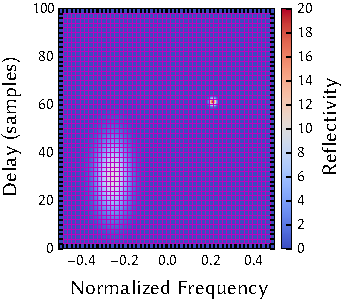
\includegraphics{range_doppler_discretization}
 \end{columns}
\end{frame}

\section{Analysis of Radar Model}

\subsection{Discrete Representation}
\begin{frame}{Model discretization from radar signal equation}
 \begin{block}{Narrow-band radar equation for received signal}
  \vspace{-2ex}
  \begin{equation*}
   y(t) = \int_0^T \int_{-\infty}^{\infty} s(t - \lambda) e^{2\pi i f (t - \lambda)} h(f, \lambda) \dee{f} \dee\lambda
  \end{equation*}
  \vspace{-2ex}
 \end{block}
 Discretization process:
 \begin{itemize}
  \item Sample measurements with time spacing $\tau$
  \item Discretize transmitted signal with spacing $\tau$ at $L$ points
  \item Discretize delay with spacing $\tau$ at $P$ points
  \item Discretize frequency with spacing $\Delta{f}$ at $N$ points
 \end{itemize}
 \begin{block}{Discretized radar model}
  \vspace{-2ex}
  \begin{equation*}
   y[m] = \sum_{p=0}^{P-1} \frac{1}{\sqrt{N}} s[m - p + L - 1] \left(\sum_{n=0}^{N-1} e^{2\pi i n m / N} h[n,p] \right)
  \end{equation*}
  \vspace{-2ex}
 \end{block}
\end{frame}

\begin{frame}{Reflectivity coefficients from function}
 From discretization process, can write the "point target" reflectivity coefficients in terms of the original function:
 \begin{equation*}
  h[n,p] = \int_{p \tau}^{(p+1)\tau} \left[h(f, \lambda) e^{2\pi i f \lambda} * b_{p + 1}(f) \right](n\Delta{f}) \dee\lambda
 \end{equation*}
 \begin{enumerate}
  \item Blur in frequency by convolving with wrapped sinc function:
  \begin{equation*}
   b_{k}(f) = \frac{1}{N} e^{-\pi i (2k + N - 1) \tau f} \frac{\sin(N \pi \tau f)}{\sin(\pi \tau f)}
  \end{equation*}
  \item Sample at discretized frequency point
  \item Integrate over delay window of discretized delay point
 \end{enumerate}
\end{frame}

\subsection{Sparsity and the Radar Model}

\begin{frame}{Representing an off-grid point target}
 Off-grid point targets are still relatively sparse!
 \begin{itemize}
  \item All coefficients outside delay window $p_t$ are zero
  \item For frequency index, behavior dictated by wrapped sinc:
 \end{itemize}
 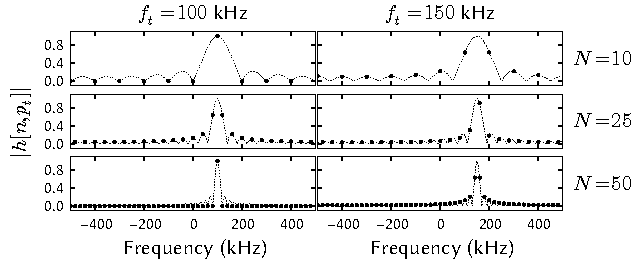
\includegraphics{point_target_coefficients}
 \begin{alertblock}{}
  Relative sparsity improves with increasing $N$\\(same number significant coefficients, many more zeros)
 \end{alertblock}
\end{frame}

\begin{frame}{Sparsity of non-point targets}
 \begin{block}{Reflectivity coefficient equation}
  \vspace{-2ex}
  \begin{equation*}
   h[n,p] = \int_{p \tau}^{(p+1)\tau} \left[h(f, \lambda) e^{2\pi i f \lambda} * b_{p + 1}(f) \right](n\Delta{f}) \dee\lambda
  \end{equation*}
  \vspace{-2ex}
 \end{block}
 \begin{itemize}
  \item Blurring from wrapped sinc mostly preserves sparsity (evidenced by point target analysis)
  \item Integration over delay exactly preserves sparsity
 \end{itemize}
 \begin{alertblock}{}
  If a target has a sparse reflectivity function, we can reasonably expect its reflectivity coefficient representation to be sparse as well.
 \end{alertblock}
\end{frame}

\section{Waveform Inversion}

\subsection{Compressed Sensing}

\begin{frame}{Under-determined systems of equations}
 Not enough measurements to constrain unknown values:
 \begin{equation*}
  {\color{purple}
  \begin{bmatrix}
   \\y\\\ 
  \end{bmatrix}}
  = 
  {\color{blue}
  \begin{bmatrix}
   &&&&&&\\
   &&&A&&&\\
   &&&&&&
  \end{bmatrix}}
  {\color{red}
  \begin{bmatrix}
   \\\\h\\\\\ 
  \end{bmatrix}}
 \end{equation*}
 \begin{center}
  {\color{purple}Measurement}\hspace{3ex}{\color{blue}Model}\hspace{3ex}{\color{red}Unknown}
 \end{center}
 \begin{itemize}
  \item Infinite number of solutions
  \item Often know that the true solution should be sparse
  \item Finding the sparsest solution is hard in general
 \end{itemize}
\end{frame}

\begin{frame}{Theory of compressed sensing}
 \begin{definition}
  \alert{Compressed sensing} is a theory to guarantee solution of an under-determined set of equations.
 \end{definition}
 \begin{block}{Approximate guidelines for application}
  \begin{itemize}
   \item Solution known to be sparse
   \item Measurements are "incoherent" (global)
   \item Minimum number of measurements on the order of the solution sparsity
  \end{itemize}
 \end{block}
 \begin{block}{Benefit}
  Can solve easy convex optimization problem instead of hard combinatorial problem
 \end{block}
\end{frame}

\begin{frame}{Equivalent convex optimization problem}
 \begin{block}{Sparsest solution to noisy measurements}
  \vspace{-2ex}
  \begin{align*}
   h^* = \quad&\argmin_h \; \left(\norm{0}{h}\right) & \norm{0}{h} =& \Bigl\lvert\left\{k : h_k \ne 0\right\}\Bigr\rvert\\
   &\:\text{s.t.} \quad \norm{2}{y - A(h)} < \eta & \norm{2}{h}^2 =& \sum_k \abs{h_k}^2
  \end{align*}
  \vspace{-2ex}
 \end{block}
 \begin{block}{$l_1$-regularized least-squares (convex)}
  \vspace{-2ex}
  \begin{align*}
   h^* = \quad&\argmin_h \; \left(\frac{1}{2}\norm{2}{y - A(h)}^2 + \lambda\norm{1}{h}\right) & \norm{1}{h} =& \sum_k \abs{h_k}
  \end{align*}
  \vspace{-2ex}
 \end{block}
\end{frame}

\subsection{Convex Optimization}

\begin{frame}{First-order methods}
 We want to efficiently solve
 \begin{equation*}
  h^* = \quad\argmin_h \; \left(\frac{1}{2}\norm{2}{y - A(h)}^2 + \lambda\norm{1}{h}\right)
 \end{equation*}
 but for systems $A$ that are too large for matrix methods.
 
 \begin{block}{First-order methods}
  \begin{itemize}
   \item Explicit matrix for $A$ not needed
   \item Only need to be able to compute $A(\cdotp)$ and $A^*(\cdotp)$
  \end{itemize}
 \end{block}
 
 \begin{alertblock}{}
  $l_1$-regularized least-squares is non-smooth because of the $l_1$ norm term, so minimizing it requires a special approach.
 \end{alertblock}
\end{frame}

\begin{frame}{First-order step}{Smooth}
 
\end{frame}

\begin{frame}{First-order step}{Non-smooth}
 
\end{frame}

\begin{frame}{The prox operator}
 The proximal operator, or \alert{prox operator}, is defined for non-smooth $G(x)$ as
 \begin{equation*}
  \mathbf{prox}_{\mu G} (v) = \argmin_{x} \; \left( G(x) + \frac{1}{2\mu} \norm{2}{x - v}^2 \right).
 \end{equation*}
 \begin{exampleblock}{Projection onto a set}
  If $G(x)$ is the indicator function for a closed convex set $\mathcal{C}$,
  \begin{equation*}
   G(x) = \begin{cases}
           0 & x \in \mathcal{C}\\
           \infty & x \notin \mathcal{C}
          \end{cases}
  \end{equation*}
$\mathbf{prox}_{G}(v)$ is projection of $v$ onto $\mathcal{C}$.
 \end{exampleblock}
\end{frame}

\begin{frame}{Proximal gradient method}
 The \alert{proximal gradient method} solves
 \begin{equation*}
  x^* = \quad \argmin_x \; \left(F(x) + G(x)\right)
 \end{equation*}
 for smooth $F(x)$ and non-smooth $G(x)$ with prox operator $\mathbf{prox}_{G}(v)$.
 \begin{block}{Algorithm}
  (Step size $\mu$) Iterate:
  \vspace{-2ex}
  \begin{align*}
   \text{Gradient step} && z^{k+1} &\coloneqq x^{k} - \mu \nabla F\left(x^{k}\right)\\
   \text{Prox step} && x^{k+1} &\coloneqq \mathbf{prox}_{\mu G}\left(z^{k+1}\right)
  \end{align*}
  \vspace{-2ex}
 \end{block}
\end{frame}

\begin{frame}{Proximal gradient method applied}
 \begin{beamercolorbox}{example text}
  Proximal gradient for $l_1$-regularized least-squares:
 \end{beamercolorbox}
 \begin{equation*}
  h^* = \quad\argmin_h \; \left(\frac{1}{2}\norm{2}{y - A(h)}^2 + \lambda\norm{1}{h}\right)
 \end{equation*}
 \begin{flalign*}
  &F(h) = \frac{1}{2}\norm{2}{y - A(h)}^2 \quad{\color{red}\Longrightarrow}\quad \nabla F(h) = -A^*\left(y - A(h)\right)\\
  &G(h) = \lambda\norm{1}{h} \quad{\color{red}\Longrightarrow}\quad
  \mathbf{prox}_{\mu G}(v) = \mathbf{soft}_{\lambda\mu}(v) = \begin{cases}
                              v - \lambda\mu, & v > \lambda\mu\\
                              0, & \abs{v} \le \lambda\mu\\
                              v + \lambda\mu, & v < -\lambda\mu
                             \end{cases}
 \end{flalign*}
 \begin{block}{Iterative Soft Thresholding}
  \vspace{-4ex}
  \begin{align*}
   \text{Matched filtering of error} && z^{k+1} &\coloneqq h^{k} + \mu A^*\left(y - A(h^{k})\right)\\
   \text{Soft thresholding} && h^{k+1} &\coloneqq \mathbf{soft}_{\lambda\mu}\left(z^{k+1}\right)
  \end{align*}
  \vspace{-3ex}
 \end{block}
\end{frame}

\begin{frame}{Iterative Soft Thresholding}
 \begin{columns}
   \column{0.6\textwidth}
   \parbox[c][0.505in]{0.45\textwidth}{\raggedright Guess:}%
   \hspace{0.05\textwidth}%
   \parbox[c][0.505in]{0.5\textwidth}{$h$}\\
   \parbox[c][0.505in]{0.45\textwidth}{\raggedright Forward model, calculate error:}%
   \hspace{0.05\textwidth}%
   \parbox[c][0.505in]{0.5\textwidth}{$z = y - A(h)$}\\
   \parbox[c][0.505in]{0.45\textwidth}{\raggedright Matched filtering of error:}%
   \hspace{0.05\textwidth}%
   \parbox[c][0.505in]{0.5\textwidth}{$A^*(z)$}\\
   \parbox[c][0.505in]{0.45\textwidth}{\raggedright Add previous guess:}%
   \hspace{0.05\textwidth}%
   \parbox[c][0.505in]{0.5\textwidth}{$h + A^*(z)$}\\
   \parbox[c][0.505in]{0.45\textwidth}{\raggedright Threshold to form new guess:}%
   \hspace{0.05\textwidth}%
   \parbox[c][0.505in]{0.5\textwidth}{$h = \mathbf{soft}(h + A^*(z))$}\\
   \column{0.4\textwidth}
   \centering
   \movie[autostart,loop,poster,width=1.85in,height=2.7in]{}{ist_animation.mp4}
 \end{columns}
\end{frame}

\begin{frame}{Accelerated proximal gradient method}
 
\end{frame}

\subsection{Implementation}

\begin{frame}{FISTA with radar model}
 Compute model with FFTW and Cython\\
 Adaptive step size
\end{frame}

\begin{frame}{Waveform inversion}
 l1-rls gives sparse solution\\
 Leaves unmodeled noise\\
 Matched filter the unmodeled noise\\
 Add noise back to sparse solution = sidelobe removal\\
 Ambiguity function is $A^*A$, so sidelobes are $(A^*A - I)$
\end{frame}

\begin{frame}{Sparse solution}
 delay-frequency figure
\end{frame}

\begin{frame}{Unmodeled noise}
 delay-frequency figure
\end{frame}

\begin{frame}{Sidelobe removal}
 delay-frequency figure
\end{frame}

\section{Results}

\subsection{Experimental Setup}

\begin{frame}{The Jicamarca incoherent scatter radar}
 \begin{itemize}
  \item Located outside Lima, Peru (equatorial ionosphere)
  \item VHF (50 MHz)
  \item Phased array of 96 $\times$\ 96 crossed half-wave dipoles
  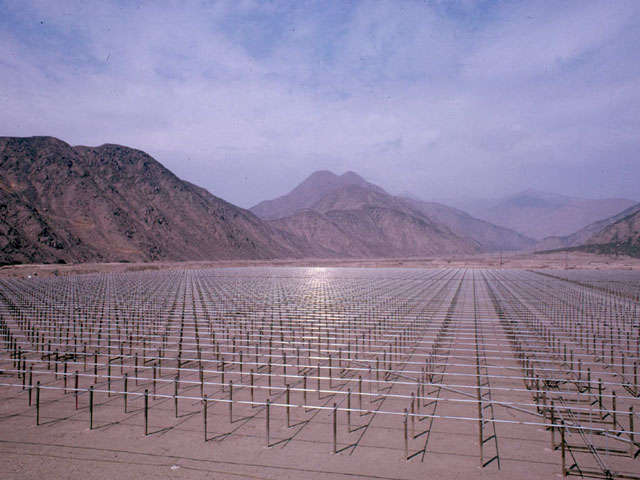
\includegraphics[height=0.4\textheight]{jicamarca}
  \item 1.1° beamwidth
  \item 1.5 MW peak power
  \item 1 MHz bandwidth (TX and RX)
  \item Interferometry and/or dual polarization receive
 \end{itemize}
\end{frame}

\begin{frame}{Jicamarca experiment goals}
 \begin{columns}
  \column{0.4\textwidth}
  \begin{block}{Goals}
   \begin{itemize}
    \item Test sparsity-based waveform inversion in \alert{crowded environment}
    \item Directly compare effectiveness of different waveforms
   \end{itemize}
  \end{block}
  \column{0.6\textwidth}
  \centering
  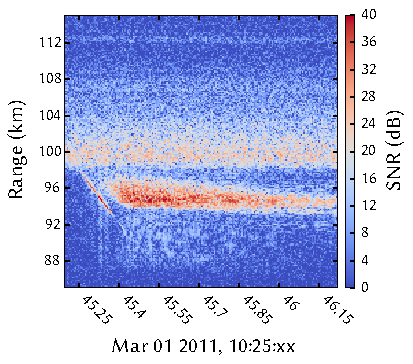
\includegraphics{ejet_head_flare_mf_rti_3}
 \end{columns}
\end{frame}

\begin{frame}{Jicamarca meteor experiment}
 \begin{columns}
  \column{0.55\textwidth}
  \begin{block}{Description}
   Alternating sequence of 5 common waveforms for observing meteor region (80-140 km altitude).
  \end{block}
  \column{0.46\textwidth}
  \begin{block}{Parameters}
   \vspace{-1.25ex}
   \begin{itemize}
    \item Pulse interval of 1 ms
    \item Sample time of 1 $\mu$s\\(150 m range resolution)
   \end{itemize}
   \vspace{-1.25ex}
  \end{block}
 \end{columns}
 \vspace{2ex}
 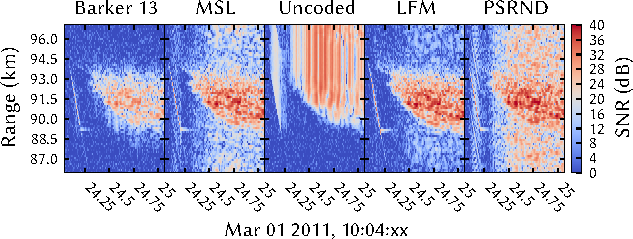
\includegraphics{head_and_flare_mf_rti_block}
\end{frame}

\subsection{Waveform Inversion}

\begin{frame}{Movie of meteor sidelobe removal}
 \movie[loop,poster,width=4.320687in,height=2.28in]{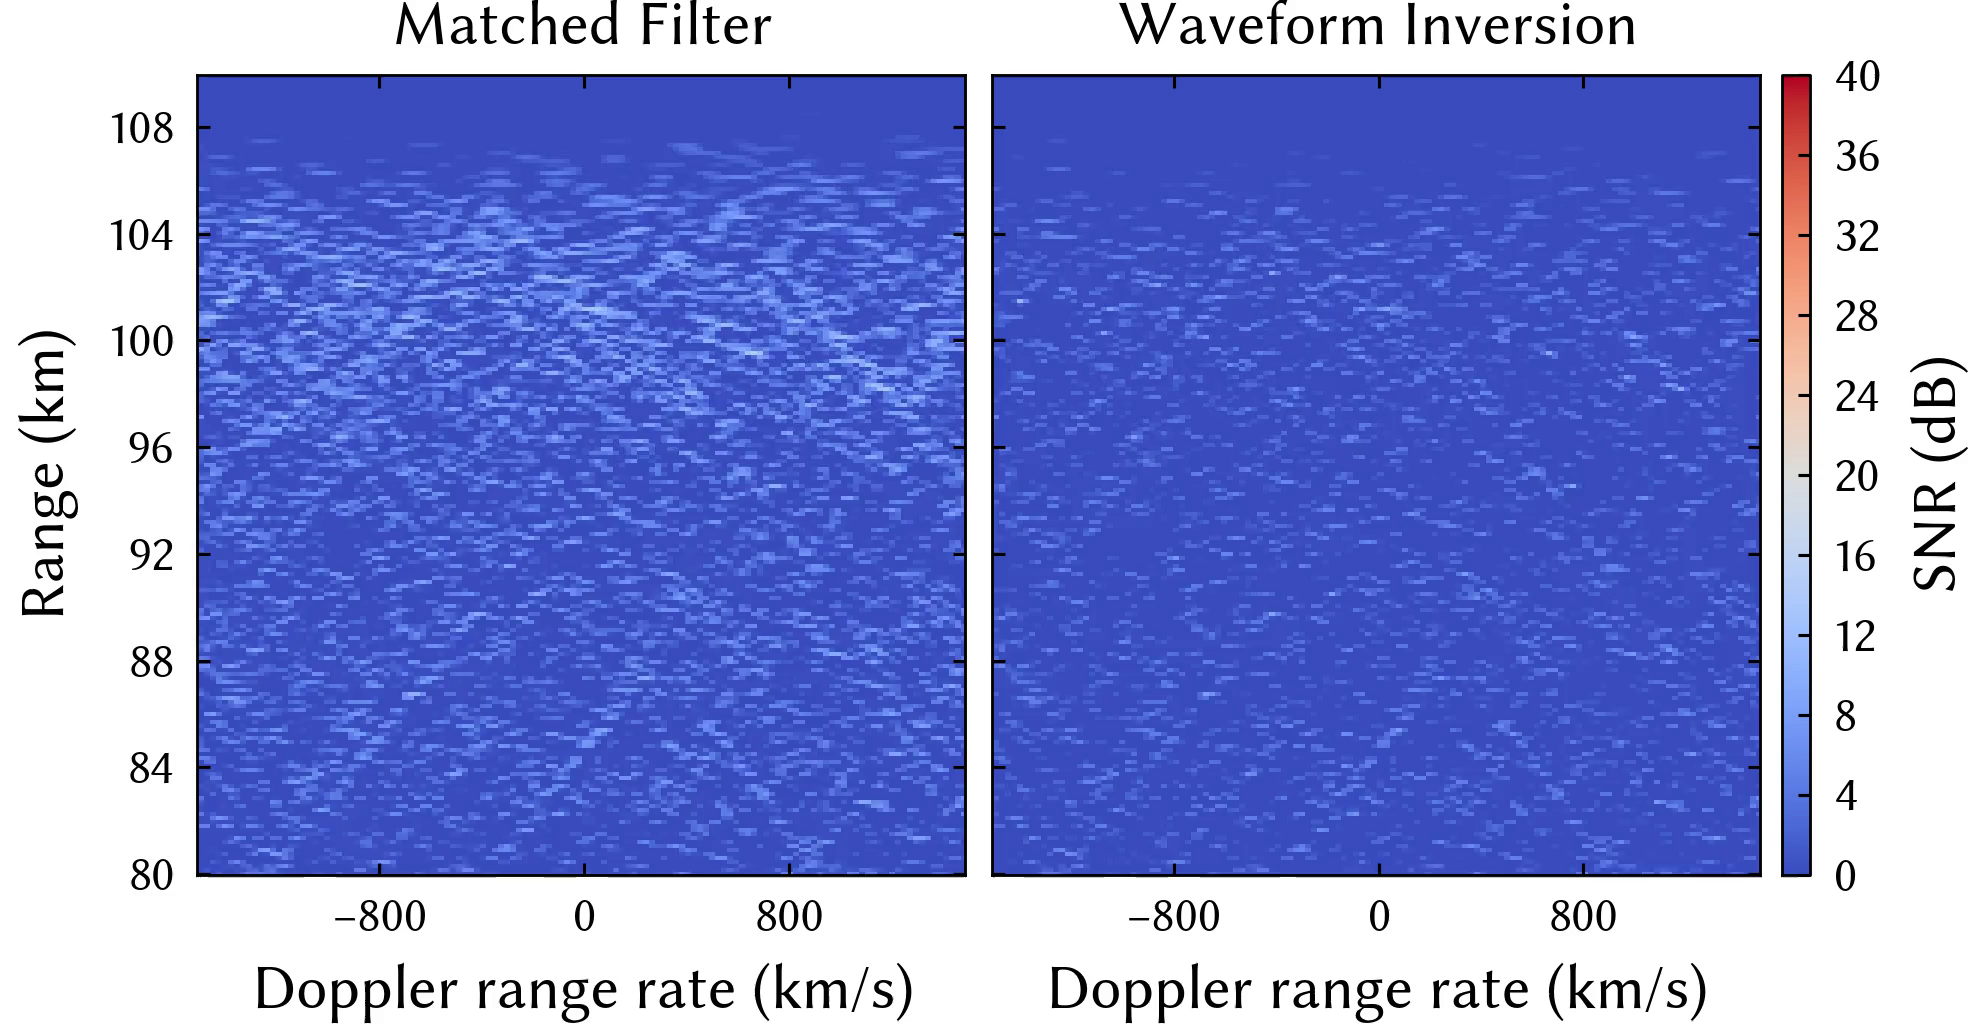
\includegraphics[width=\textwidth]{head_and_flare_mf_vs_recovered_1}}{head_and_flare_mf_vs_recovered_1.mp4}
\end{frame}

\begin{frame}[t]{Example: Minimum sidelobe code}
 \begin{tikzpicture}
  \tikzstyle{every node}=[minimum width=\widthof{Waveform}+2ex]
  \node[left,align=center] at (0,0.5) {Matched\\Filter};
  \node[right,image] at (0,0) {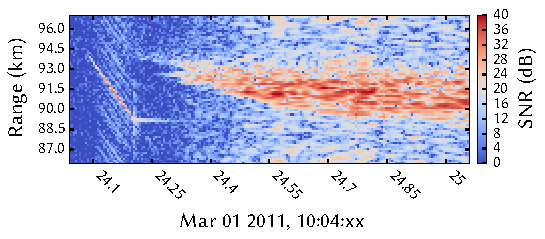
\includegraphics{head_and_flare_mf_rti_1}};
  \fill[white] (0,-1.125) rectangle (9,-0.875);
  \node[left,align=center] at (0,-2.3) {Waveform\\Inversion};
  \node[right,image] at (0,-2.8) {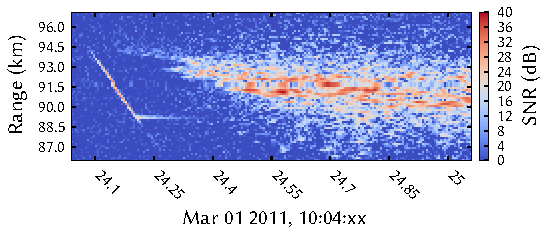
\includegraphics{head_and_flare_recovered_rti_noise_1}};
 \end{tikzpicture}
\end{frame}

\begin{frame}[t]{Example: Barker-13 code}
 \begin{tikzpicture}
  \tikzstyle{every node}=[minimum width=\widthof{Waveform}+2ex]
  \node[left,align=center] at (0,0.5) {Matched\\Filter};
  \node[right,image] at (0,0) {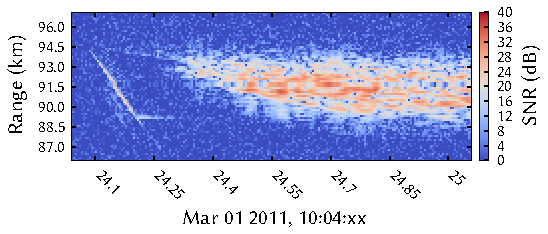
\includegraphics{head_and_flare_mf_rti_0}};
  \fill[white] (0,-1.125) rectangle (9,-0.875);
  \node[left,align=center] at (0,-2.3) {Waveform\\Inversion};
  \node[right,image] at (0,-2.8) {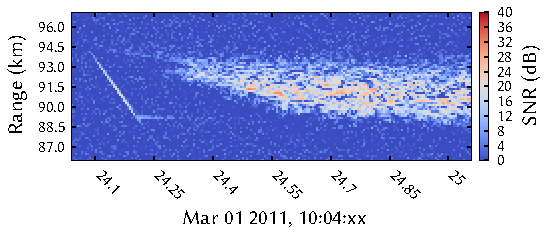
\includegraphics{head_and_flare_recovered_rti_noise_0}};
 \end{tikzpicture}
\end{frame}

\begin{frame}[t]{Example: Pseudorandom code}
 \begin{tikzpicture}
  \tikzstyle{every node}=[minimum width=\widthof{Waveform}+2ex]
  \node[left,align=center] at (0,0.5) {Matched\\Filter};
  \node[right,image] at (0,0) {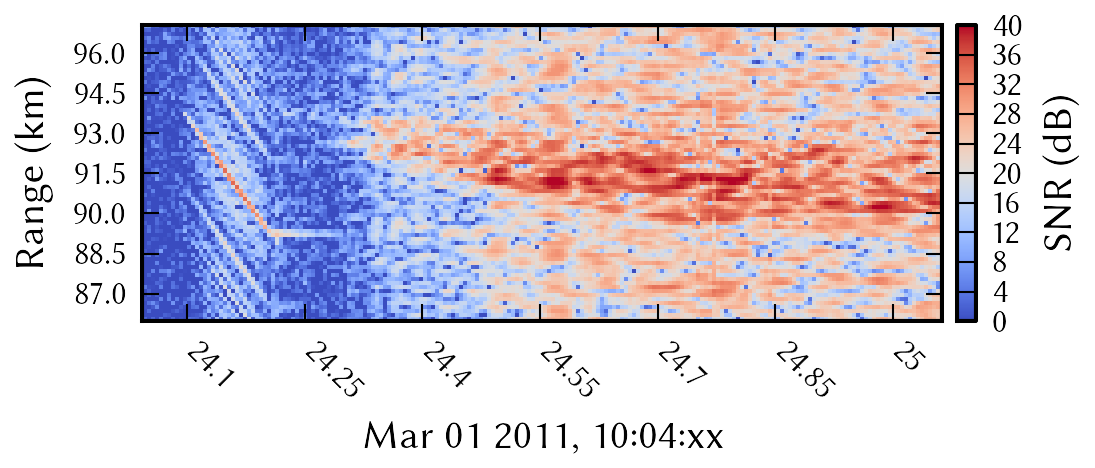
\includegraphics{head_and_flare_mf_rti_4}};
  \fill[white] (0,-1.125) rectangle (9,-0.875);
  \node[left,align=center] at (0,-2.3) {Waveform\\Inversion};
  \node[right,image] at (0,-2.8) {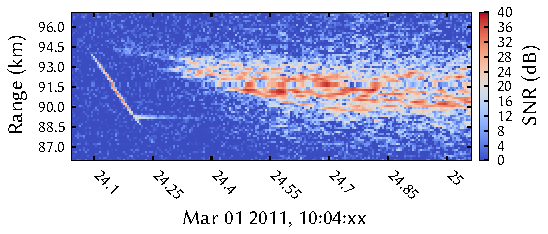
\includegraphics{head_and_flare_recovered_rti_noise_4}};
 \end{tikzpicture}
 \vspace{-5ex}
 \begin{alertblock}{}<2>
  Works with variety of codes
 \end{alertblock}
\end{frame}

\begin{frame}[t]{Example: LFM chirp}
 \begin{tikzpicture}
  \tikzstyle{every node}=[minimum width=\widthof{Waveform}+2ex]
  \node[left,align=center] at (0,0.5) {Matched\\Filter};
  \node[right,image] at (0,0) {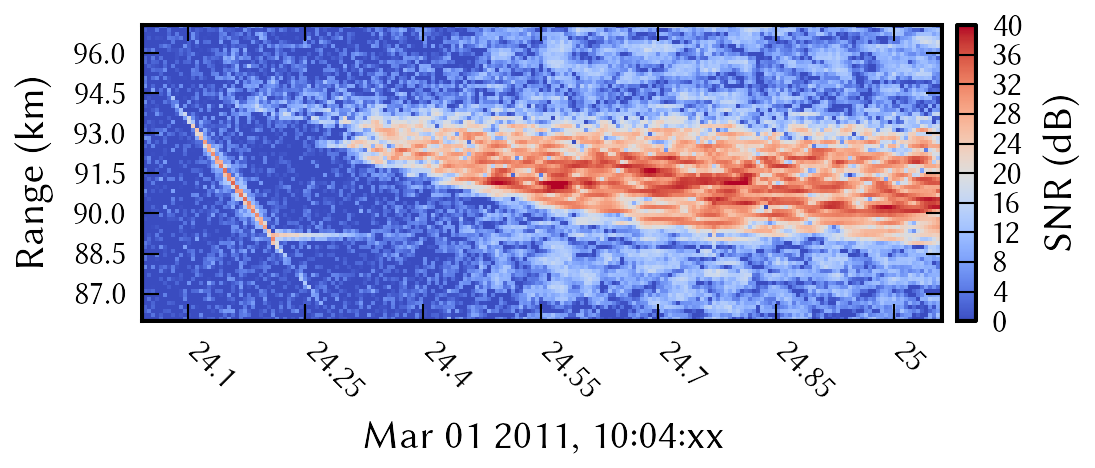
\includegraphics{head_and_flare_mf_rti_3}};
  \fill[white] (0,-1.125) rectangle (9,-0.875);
  \node[left,align=center] at (0,-2.3) {Waveform\\Inversion};
  \node[right,image] at (0,-2.8) {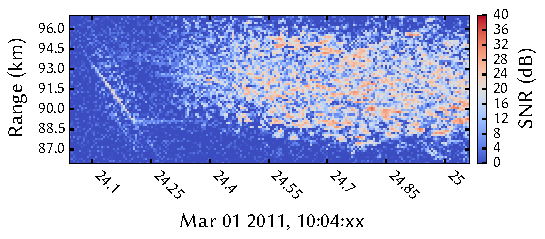
\includegraphics{head_and_flare_recovered_rti_noise_3}};
 \end{tikzpicture}
 \vspace{-5ex}
 \begin{alertblock}{}<2>
  Some codes are troublesome
 \end{alertblock}
\end{frame}

\begin{frame}[t]{Example: Uncoded}
 \begin{tikzpicture}
  \tikzstyle{every node}=[minimum width=\widthof{Waveform}+2ex]
  \node[left,align=center] at (0,0.5) {Matched\\Filter};
  \node[right,image] at (0,0) {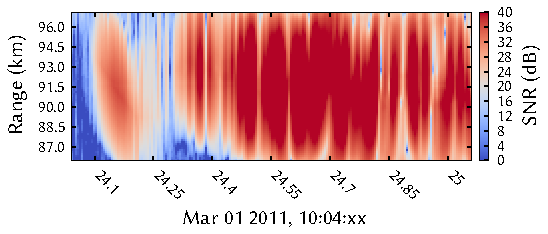
\includegraphics{head_and_flare_mf_rti_2}};
  \fill[white] (0,-1.125) rectangle (9,-0.875);
  \node[left,align=center] at (0,-2.3) {Waveform\\Inversion};
  \node[right,image] at (0,-2.8) {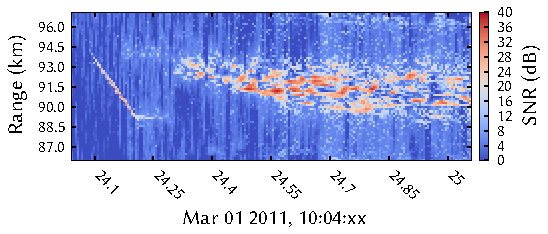
\includegraphics{head_and_flare_recovered_rti_noise_2}};
 \end{tikzpicture}
 \vspace{-5ex}
 \begin{alertblock}{}<2>
  Works even with uncoded pulses!
 \end{alertblock}
\end{frame}

\begin{frame}[t]{Waveform inversion code comparison}
 \begin{tikzpicture}
  \tikzstyle{every node}=[minimum width=\widthof{Waveform}+2ex]
  \node<1>[left,align=center] at (0,0.5) {Minimum\\sidelobe};
  \node<1>[right,image] at (0,0) {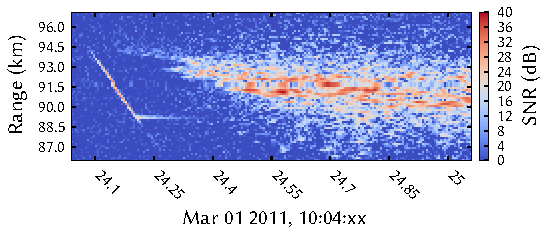
\includegraphics{head_and_flare_recovered_rti_noise_1}};
  \node<2->[left,align=center] at (0,0.5) {Pseudo-\\random};
  \node<2->[right,image] at (0,0) {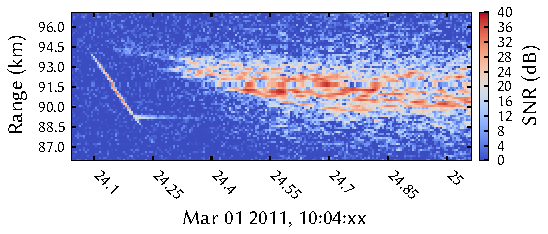
\includegraphics{head_and_flare_recovered_rti_noise_4}};
  \fill[white] (0,-1.125) rectangle (9,-0.875);
  \node[left,align=center] at (0,-2.3) {Uncoded};
  \node[right,image] at (0,-2.8) {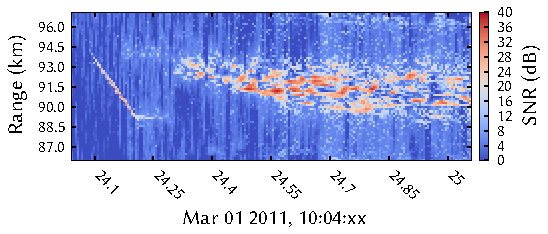
\includegraphics{head_and_flare_recovered_rti_noise_2}};
 \end{tikzpicture}
 \vspace{-5ex}
 \begin{alertblock}{}<3->
  Quality of solution depends on fidelity of waveform
 \end{alertblock}
\end{frame}

\section{Conclusion}

\begin{frame}<beamer>{Outline}
 \tableofcontents[currentsection,hideallsubsections]
\end{frame}

\againframe<5->{contributions}

\begin{frame}{Acknowledgements}
 
\end{frame}

\appendix

\begin{frame}{Linearized ADMM}
 
\end{frame}

\end{document}
